\section{Sensibility Testbed Architecture}\label{sec-design}

As stated in Section~\ref{sec-overview}, the architecture of Sensibility 
Testbed involves three interacting parties:  
%as shown in Figure~\ref{fig-arch}: 
researchers, a clearinghouse server, and mobile device owners. In this section, we 
%discuss the role and functions of each party, and introduce their key 
%techniques. We 
use the same example as in 
Section~\ref{sec-walkthrough} to explain the interaction between these 
parties, where researcher Bob wants to know the cellular service quality 
using Alice's device.

%\begin{figure}
%\center{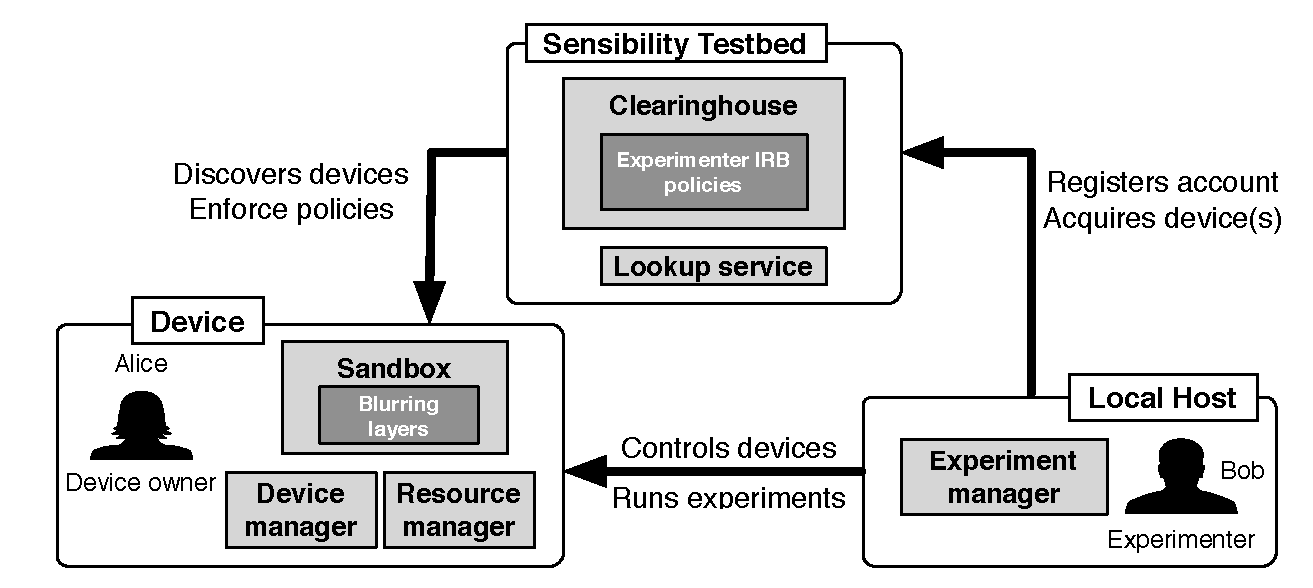
\includegraphics[width=\columnwidth]{figs/arch.pdf}}
%%\vspace*{-20pt}
%\caption{\small Sensibility Testbed architecture. \label{fig-arch}}
%\end{figure}

\subsection{Researcher Specifies IRB Policies}\label{sec-ch}
Before conducting any experiments, Bob first registers an account 
at the clearinghouse. 
The clearinghouse~\cite{ch} is a testbed server that has two 
responsibilities. First, it keeps track of devices and grants 
researchers access to available devices; and second, it
sets up the relevant IRB policies on behalf of the researcher, that 
must be enforced on remote devices.
%It allows experimenters to register accounts and share 
%access to a common pool of devices.

To register his experiment, Bob first fills out a form on the clearinghouse 
web page, which has a list of checkboxes for all available sensors 
and text boxes indicating the precision and frequency at which Bob 
desires to access 
each sensor. Bob checks off only the sensors necessary for his experiment, 
and sets the policies by filling in the text boxes for each sensor.
In this case, Bob specifies that 
his experiment can (1) read location information
from devices at the granularity of a city, (2) read accurate
cellular signal strength and network type, as well as
cell IDs, and (3) get location and
cellular network data updates every 10 minutes. 
%Bob then downloads documents to provide to his IRB that 
%explains the details about his experiment, \sysname and the technical 
%restrictions his experiment will have. Bob then obtains IRB approval at 
%his institution, provides his institution's IRB policies to the 
%\sysname website, and signs up for his experiment. 
After filling out this form, Bob downloads the experiment description 
he provided, the detailed information about \sysname's approved IRB, 
and several relevant forms, such as those addressing consent 
(Section~\ref{sec-repy}), terms of participation (for device owners),  
terms of usage (for the researcher), and so on.  
Bob then uses these forms as a template to complete the IRB application 
with his institution. These forms serve as a set of reference documents 
to make it easier for researchers like Bob to 
file the necessary IRB paperwork with their institutions.

The form that Bob filled out on the clearinghouse website is used to
enforce a set of technical restrictions for his experiment. 
The blurring layers are provided by 
\sysname, and are set up in a non-bypassable fashion -- it is not 
Bob's task to implement the approved access policies. This means
that even if Bob makes an error in his code or his code is malicious, his 
experiment is still restricted in the data it can acquire. 
Therefore, Bob's IRB 
policies which request access to cellular signal strength and network type, would result 
in his experiment being blocked from reading the cellular roaming status and area 
code. Note that the latter information is accessible with the same 
Android permission, but is blocked by \sysname. 
After the application is submitted, Bob's IRB may disagree with 
his initial experiment requirements. For example, Bob's IRB will not permit
his experiment to access cell IDs in cellular networks, but 
approves the other policies. 
%Bob wants to access cell 
%IDs in cellular networks, but his IRB disallows such data access. Bob then
In this case, Bob will revise the experiment registration form, refile the paperwork, 
and obtain IRB approval. Bob then submits the revised  
registration form and his IRB approval to the clearinghouse.

 When an account is approved, Bob 
% is assigned a pair of public/private \textit{authentication keys} by the 
%clearinghouse, to authenticate himself with the clearinghouse. This
%researcher 
can sign into the clearinghouse and request a 
number of sandboxes for his experiment. The clearinghouse 
looks up available sandboxes on behalf of Bob. If Alice's device is discovered, the 
clearinghouse stores her device's meta information (an anonymized 
key), %\textit{identification key}, 
and assigns her device to Bob's experiment account. 

The clearinghouse creates a list of sensor access policies for Bob's
experiment, according to Bob's specified IRB policies. The 
clearinghouse parses Bob's registration form, extracts each sensor name, 
data accuracy and access frequency limits as the 
input parameters to the blurring layer code (to blur an exact location 
to a city center, disallow access to cell IDs, and allow cellular network and 
location query once every 10 minutes). Finally, the clearinghouse 
instructs Alice's device to implement these IRB policies. The involvement 
of the clearinghouse in any given experiment ends at this point.
It does not store any data on the researcher's behalf. 

%Besides assigning devices, the clearinghouse also has the role of 
%instructing the sandboxes assigned to this researcher to add the IRB 
%policies specified during registration. The clearinghouse does so 
%by communicating with the resource managers on those devices, which 
%control the code executed in the sandboxes. 

%However, it can direct the release of data to a server designated by the 
%researcher. To do so, the experimenter must register
%his server by providing its certificate and URL to the
%clearinghouse, which will then instruct the devices
%accessible to the experimenter that all the sensor data collected should be
%sent to this server. The sandboxes on these devices will issue
%\texttt{HTTPS POST} using the server's certificate, and send encrypted
%data to the experimenter's server.

%The key role of this component is to facilitate device sharing, 
%which relieves individual experimenters from repeatedly 
%recruiting devices for each experiment.
%
%Note that in Sensibility Testbed, there are two types of keys. A device
%owner has an \textit{identification key} to identify the app installed on a 
%device. This key is mostly used by a lookup service. 

%This pair of keys are mostly used by the clearinghouse and 
%experiment manager.

%\lois{have you introduced the idea of keys yet? If not, I think this needs to be explained.}

\subsection{Device Onwner's Informed Consent and Privacy Policy 
Enforcement}\label{sec-repy}

In order for Alice to participate in Sensibility Testbed as a device owner,
she starts by installing the Sensibility Testbed app from 
the Android app store~\cite{sensibility-app}. The app includes all the device
software for Alice to give informed consent, configure the permission she
is comfortable with, and for Bob's experiment code to conform to the 
IRB policies at the clearinghouse when running on Alice's device.

\subsubsection{Informed Consent}\label{subsec:informed-consent}

After downloading the app, it informs Alice about the testbed's usage and 
privacy policy in a consent form and must give consent before participating.
The usage policy requires that the participants in \sysname must be at least 
18 years old, and do not belong to protected group such as pregnant women.
Any other device owner, regardless of country or background, can 
opt into our testbed in this manner, and can opt out just by uninstalling the app. 
If Alice agrees, the app will be installed on her device, which includes other
device software that enforces Bob's IRB policies specified at the 
clearinghouse (Section~\ref{sec-bob-policy}), and allows Alice to set her 
own policies (Section~\ref{sec-alice-policy}).


\subsubsection{Blurring Layers for IRB Policies}\label{sec-bob-policy}

\begin{figure}
\center{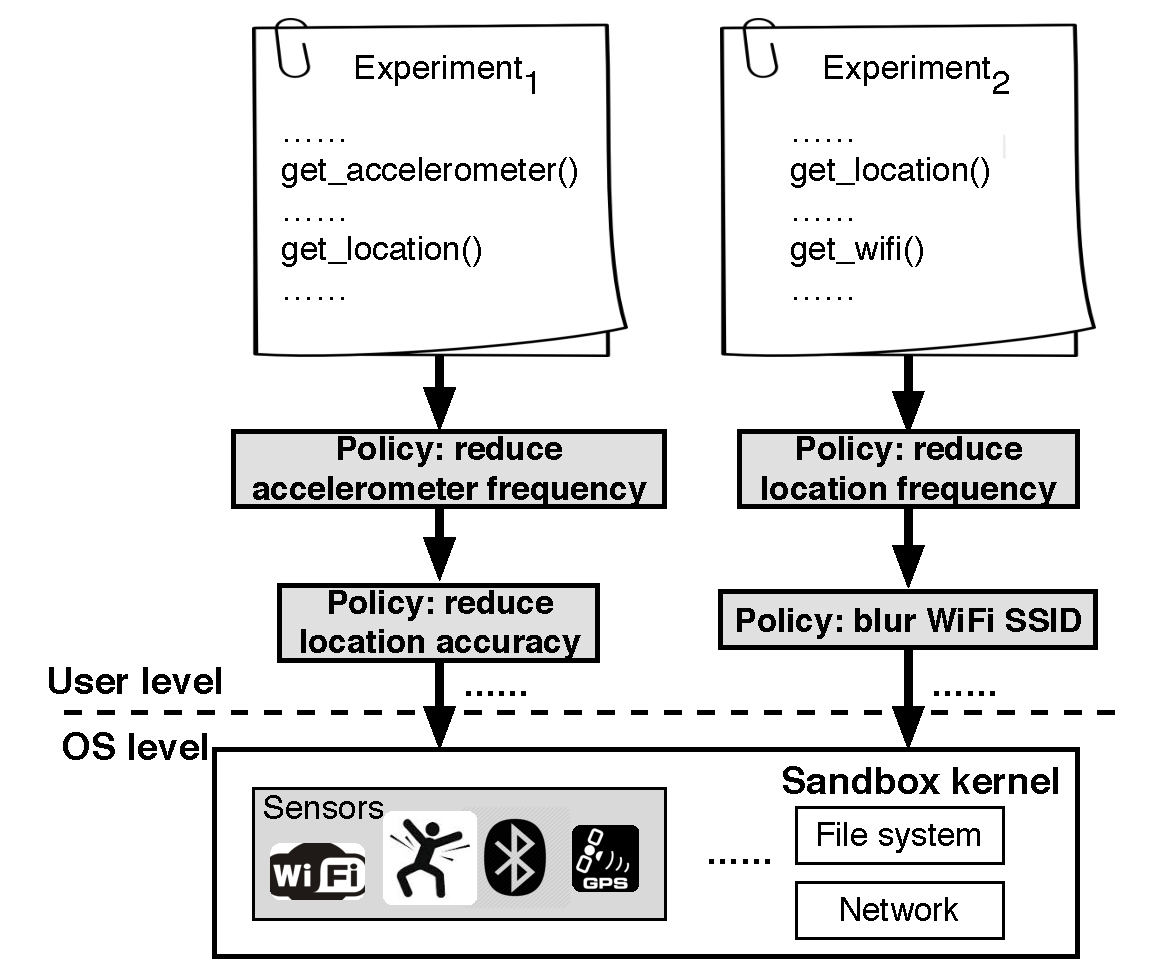
\includegraphics[width=0.9\columnwidth]{figs/blur.pdf}}
%\vspace*{-20pt}
\caption{\small Policy stack demonstrating how Sensibility Testbed implements blur policies.
\label{fig-blur}}
\end{figure}

Bob's IRB policies are implemented as blurring layers in a secure sandbox, with 
each layer enforcing an access control policy over a sensor on Alice's device. 
The sandbox in \sysname (Section~\ref{sec-sandbox}) provides a list of system 
calls to experiment code, such as \path{get_location()}, \path{get_accelerometer()}. 
Using a system call interposition technique in our prior work~\cite{cappos2010retaining}, 
the sandbox can interject code to control the behavior of these calls. Using this 
technique, a sensor access policy can (1) reduce the precision of the raw sensor data 
returned from a device, such as returning the location of a nearest city rather than the 
device's exact location, and (2) restrict the frequency of access to a sensor, such as the 
access rate of a gyroscope or an accelerometer, to avoid password 
interference~\cite{michalevsky2014gyrophone}.

%and (3) disable  
%access to a certain sensor in sensitive situations, such as 
%turning off a camera when a device is in a residential or work area.
%Implementation of the last policy is still ongoing, so this paper will mainly address
%how blurring layers allow for the execution of the first two types of policies. 

%The sandbox kernel determines how IRB policies are implemented by affecting system calls. It can
%interpose on a call and modify the data returned, or control the frequency with which a call can be made over
%a period of time. 

%Different policies implemented can be stacked in tandem to 
%control different sensor accesses, like in Figure~\ref{fig-blur}.
%As mentioned above, Bob provided his IRB policies through our clearinghouse.
%Before Bob runs his experiment, the clearinghouse loads the access policies and instructs the sandbox on Alice's device to
%restrict sensor access accordingly. 
%
%Using the \path{get_location()} call as an example, 
%when Bob's code requests location data from Alice's device, the Repy sandbox first
%invokes the location-related Android code. 
%%(line 10 in Figure~\ref{fig-getlocation}). 
%When the location data is returned, according to Bob's IRB policy
%indicates that the returned location coordinates should be blurred to the nearest city to Alice's
%device, instead of her actual location. As a result, 
%For example, the sandbox returns a perturbed location that is less accurate, 
%%Furthermore, as Bob's IRB policy disallows collecting information about cell tower IDs, 
%%blocks any access to cell IDs, 
%%by another policy. Similarly, other information
%blurs a WiFi SSID to a hashed string, and restricts the frequency to access a
%gyroscope to prevent inferring passwords~\cite{michalevsky2014gyrophone}, and so on. 
\textbf{Reducing Data Precision.}
Each blurring layer defines one of the above two categories of policies. 
For example, to blurr Alice's location to a nearest city, the following layer
will be instantiated by the sandbox, as instructed by the clearinghouse:

\begin{Verbatim}
1. \textcolor{Purple}{def} \textbf{\textcolor{NavyBlue}{get_city_location}}():
2.   \textcolor{BrickRed}{"""}
3.   \textcolor{BrickRed}{This function replaces the exact coordinates of} 
4.   \textcolor{BrickRed}{the Android device with the coordinates for the } 
5.   \textcolor{BrickRed}{geographic center of the nearest city.}
6.   \textcolor{BrickRed}{"""}
7.
8.   exact_location = get_location()
9.   city_location = find_closest_city(exact_location)
10.  \textcolor{Purple}{return} city_location
11.
12. \textcolor{BrickRed}{# Substitute get_location with get_city_location.}
13. \textbf{CHILD_CONTEXT_DEF[\textcolor{BrickRed}{"get_location"}] = \{}
14.    \textbf{\textcolor{BrickRed}{"target"}: get_city_location,}
15. \textbf{\}}
\end{Verbatim}

As a result, whenever Bob's experiment code calls \path{get_location()}, 
the blurring layer above replaces it with \path{get_city_location()}. Therefore,
this blurring layer guarantees Bob's IRB policy.

\textbf{Restricting Data Access Frequency.}
These policies can be implemented in a similar way. When an experiment 
program's use of a sensor is above a given threshold, the blurring layer 
pauses the code for as long as required to bound it, on average, below 
the threshold. Therefore, if an experiment attempts to use a sensor at a 
rate faster than is allowed by a policy, the system call is blocked until 
sufficient time has passed to average out the overall access rate. An example
of this blurring layer that restricts location queries to be once per 10 minutes
is given in our technical report~\cite{zhuangTR15}.

Both the type of blurring layer (blur location to the nearest city) and the 
parameters to each layer (access location once per 10 minutes) are parsed
by the clearinghouse from Bob's input, and passed on to the sandbox on 
Alice's device. Each blurring layer is implemented as templated code, 
pre-loaded in each sandbox, and can be instantiated with parameters 
once the clearinghouse instructs it to do so.

\textbf{Policy Stack.}
Different sets of policies can be customized 
according to the regulations set by Bob's IRB, through loading 
individual blurring layers in order, as a policy stack. In each stack, 
a lower layer is the ancestor of a higher layer. Every layer inherits 
the policy defined by its ancestor layers, with the exception of the lowest layer. 
%Each blurring layer is untrusted by its ancestor layers, 
%but is trusted by its descendant layers. \yanyan{maybe cut this.}
The lowest blurring layer with no ancestors is the 
Sensibility Testbed's sandbox kernel. The experiment program runs at the top 
of the policy stack, thereby inheriting all the policies defined by the
lower layers, as shown in Figure~\ref{fig-blur}. 
Each policy stack acts as a set of filters for different sensors, through 
which a call must pass before a sandboxed program can
access the sensor data. 
%Different stacks can be customized for different IRB policies.

When Bob starts his experiment, the sandbox %uses its blurring layer creation call to 
instantiates the first blurring layer according to its contract, i.e., the function 
mapping that contains the kernel's exported functions.
%the security layer instantiation call, and the remaining
%command-line arguments. 
The newly instantiated blurring layer repeats this process 
%using the 
%encasement library's
%blurring layer creation call 
to instantiate the next security layer with a potentially updated contract and 
function mapping. Eventually, Bob's program is instantiated
in a separate layer with the functions provided
through the stack of blurring layers that preceded it.
Bob's program will then be subject to all the 
policies defined in the preceding layers, or the policy stack. 
As a result,  the policies are transparently applied to Bob's experiment code. 

This mechanism is transparent to the experimenters 
and device owners, as the implementation of policies is controlled by the 
clearinghouse on behalf of the experimenters. An experimenter is aware 
of certain policies in place, but does not need to implement or explicitly
enforce such policies. 
\jill{we should add something in this example about how default policies play a role}
\yanyan{Can we explain how some policies supersede other policies? ie, device
owner's policies > \sysname default policies > researcher's IRB policies.}
%In the following, we describe how to implement each blurring layer, 
%and use them to form a policy stack.

\subsubsection{Device Owner's Policies}\label{sec-alice-policy}
A device manager is a part of the device software that 
allows device owners to control the software running on their 
devices. With the device manager, Alice thus can install and remove 
all the other device software, opt in and out of any experiment, 
and set permissions to access the sensors on Alice's device. 

When the \sysname app is started on Alice's device, the device 
manager interface displays a list of running experiments and their policies. If 
Alice does not agree with any policy, she can opt out of the particular 
experiment using the device manager interface. 

Alice can also configure the policies through the device manager to allow
sensors on her device to be acessed at a granularity she is comfortable with.
Alice sets these policies via the user interface of the \sysname app. 
The device manager then parses them just as the clearinghouse
parses Bob's IRB policies, and then passes the policies on to the sandbox.
The implementation of Alice's policies is the same as Bob's, through
the use of blurring layers.
These policies supersede any policies set by researcher's IRB. For 
example, if Alice disallows access to her location information, then 
Bob's experiment cannot get any location from Alice's device even
Bob's IRB allows this access. 


\subsection{Researcher Conducts an Experiment}\label{sec-emt}

%The last component in the testbed is an experiment manager, which 
To run code on Alice's device, Bob needs to download an experiment 
manager to his own computer.
Bob uses the experiment manager as a light-weight command line 
console~\cite{demo-kit} to directly access Alice's device, upload 
experiment code, and %written in the Repy programming interface, and
communicate with Alice's device to start or stop the execution of the experiment. 
%To authenticate himself with the remote sandbox, the researcher uses 
%his public/private key pairs to establish a secure connection from his
%computer. 
The experiment manager can also be used to download data 
from the remote devices to Bob's local computer, or
Bob can set up his own server to store the data\footnote{\scriptsize
If a researcher stores data on his own server, he must use protective
measures to ensure that data sent from the mobile devices is
properly encrypted, and the server storage cannot be tampered
with by any other parties. This is enforced by requiring the experimenter to register
his server by providing its certificate and URL to our
clearinghouse. Following receipt of this data, the clearinghouse will instruct the devices
accessible to the experimenter that all the sensor data collected should be
sent to this server. The sandboxes on these devices will issue
\texttt{HTTPS POST} using the server's certificate, and send encrypted
data to the experimenter's server.}. 
If Bob stores data on his own server, he must use protective
measures to ensure that data sent from the mobile devices is
properly encrypted, and the server storage cannot be tampered
with by any other parties. Researchers can also opt to use a data 
store service we provide (a service called Sensevis~\cite{sensevis}). 
After the data is collected, the method of 
securely storing the data will be mandated by Bob's IRB.

\smallskip
This Sensibility Testbed clearinghouse protocol for research plays a central role in
easing the process of device recruitment and experiment setup for experimenters, 
and ensures the enforcement of privacy policies. 
%Prior to running an experiment on Sensibility Testbed, a
%experimenter first fills out a form in plain text to describe the
%purpose of the research experiment. This experiment description
%is created at the Sensibility Testbed clearinghouse
%where the researcher indicates the type of data to be collected,
%how that data will be used and stored, and so on. 
%
%Once this information is collected from the researcher, the
%clearinghouse automatically generates a set of blurring layers
%that implements the experiment policy (Section~\ref{sec-policy}). In
%Sensibility Testbed, researchers can collect data from the
%sensors on the device, such as GPS, Bluetooth, battery
%information, accelerometer, light, and orientation,
%etc. The blurring layers we provide consist of
%data access restrictions, created in accordance with
%researcher's experiment description, by using the Sensibility
%Testbed's sandboxing technique 
%(Section~\ref{sec-repy})~\cite{cappos2010retaining}. These restrictions ensure that
%the researcher cannot conduct experiments to access data that
%extend beyond the experiment policy. 
%
%This Sensibility Testbed
%clearinghouse protocol for research plays a central role in
%easing the approval process of IRB, and ensures the enforcement
%of privacy policy\footnote{The Sensibility Testbed Clearinghouse
%protocol for research with human subjects has been approved by
%the IRB at New York University. \yanyan{might need a link to
%your approval letter or ref number}}. 
Using Sensibility Testbed, device owners' privacy is protected
from any inadvertent or malicious attempt, and researchers 
are able to go through a streamlined process of device 
recruitment and experiment setup.

